% star stencils
%
% stars drawn in TikZ
% cut into painter's tape on a laser CNC
% to be used as a stencil to paint onto the ceiling of a child's room


\documentclass[]{book}

\usepackage[
    paperwidth=1.89in,  % tape is 1.89" wide
    paperheight=11in,   % tape is applied to a board 11" long
    top=0.5in,
    bottom=0.6in,       % help roughly center the stars
    left=0.25in,
    right=0.25in
]{geometry}

\usepackage{tikz}
\usetikzlibrary{shapes,backgrounds}

\pagenumbering{gobble}  % laser cnc has trouble w/ text

\makeatletter
\@openrightfalse        % open left to compare the 2 pages left/right in viewer
\makeatother



\newcommand{\sep}{\vskip14mm}  % add space between stars so the tape doesn't tear
\newcommand{\scale}{0.3937}    % 1 cm = 1 inch

% SEE
% https://tex.stackexchange.com/questions/58903/how-to-draw-star-in-tikz-background
\newcommand{\tstar}[5]{
% inner radius, outer radius, tips, rot angle, options
\pgfmathsetmacro{\starangle}{360/#3}
\draw[#5] (#4:#1)
\foreach \x in {1,...,#3}
{ -- (#4+\x*\starangle-\starangle/2:#2) -- (#4+\x*\starangle:#1)
}
-- cycle;
}


% two 8 point stars, the second smaller and rotated 45
\newcommand{\dstar}[5]{
% inner radius, outer radius, rot angle, options, innerscale
\pgfmathsetmacro{\starangle}{360/4}
\begin{scope}
\draw[#4] (#3:#1)
\foreach \x in {1,...,4}
{ -- (#3+\x*\starangle-\starangle/2:#2) -- (#3+\x*\starangle:#1)}
-- cycle;
\end{scope}
\begin{scope}[rotate=\starangle/2, scale=#5]
\draw[#4] (#3:#1)
\foreach \x in {1,...,4}
{ -- (#3+\x*\starangle-\starangle/2:#2) -- (#3+\x*\starangle:#1)}
-- cycle;
\end{scope}
}


\newcommand{\ngram}[4]{% outer radius, tips, rot angle, options
\pgfmathsetmacro{\starangle}{360/#2}
\pgfmathsetmacro{\innerradius}{#1*sin(90-\starangle)/sin(90+\starangle/2)}
\tstar{\innerradius}{#1}{#2}{#3}{#4}
}


% % % % % % % % % % % % % % % % % % % % % % % % % % % % % % % % % % % % %
\begin{document}


\begin{centering}


\begin{tikzpicture}[]
    \tstar{0.7}{1.6}{5}{-18}{thick}  % 5 points
\end{tikzpicture}
\sep


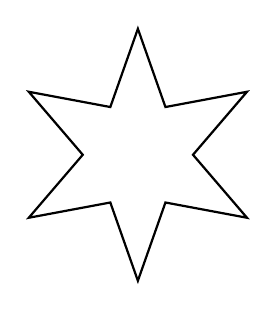
\begin{tikzpicture}
    \tstar{0.7}{1.6}{6}{0}{thick}  % 6 points
\end{tikzpicture}
\sep


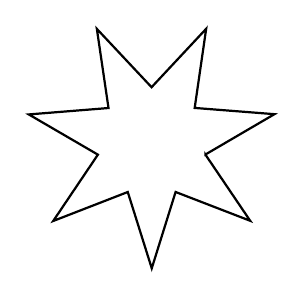
\begin{tikzpicture}
    \tstar{0.7}{1.6}{7}{-12.8}{thick}  % 7 points
\end{tikzpicture}
\sep


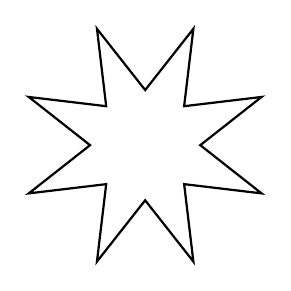
\begin{tikzpicture}
    \tstar{0.7}{1.6}{8}{0}{thick}  % 8 points
\end{tikzpicture}
\sep


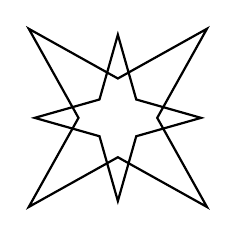
\begin{tikzpicture}
    \dstar{0.5}{1.6}{0}{thick}{0.66}  % double
\end{tikzpicture}
\sep

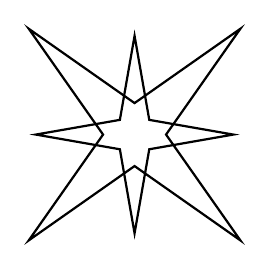
\begin{tikzpicture}
    \dstar{0.4}{1.9}{0}{thick}{0.66}  % double
\end{tikzpicture}
\sep

\end{centering}




\begin{centering}


\begin{tikzpicture}[]
    \tstar{0.6}{1.6}{5}{-18}{thick}  % 5 points
\end{tikzpicture}
\sep


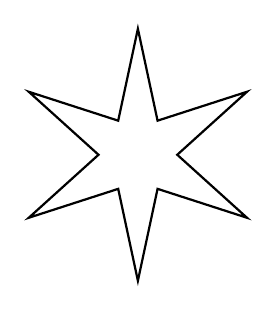
\begin{tikzpicture}
    \tstar{0.5}{1.6}{6}{0}{thick}  % 6 points
\end{tikzpicture}
\sep


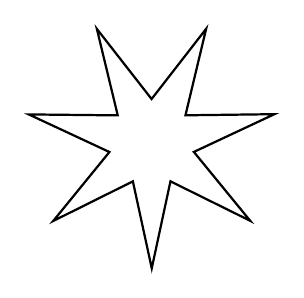
\begin{tikzpicture}
    \tstar{0.55}{1.6}{7}{-12.8}{thick}  % 7 points
\end{tikzpicture}
\sep


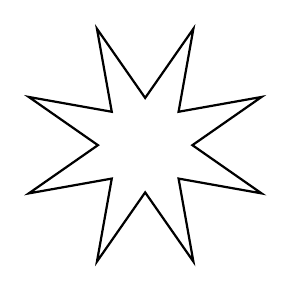
\begin{tikzpicture}
    \tstar{0.6}{1.6}{8}{0}{thick}  % 8 points
\end{tikzpicture}
\sep


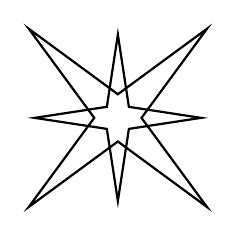
\begin{tikzpicture}
    \dstar{0.3}{1.6}{0}{thick}{0.66}  % double
\end{tikzpicture}
\sep

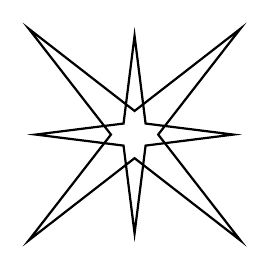
\begin{tikzpicture}
    \dstar{0.3}{1.9}{0}{thick}{0.66}  % double
\end{tikzpicture}
\sep

\end{centering}



\end{document}
